\documentclass[11pt,fullpage]{article}
%\documentclass[runningheads, letter]{llncs}
%\documentclass{llncs}
\usepackage{epsfig,longtable}
\usepackage{epsfig} 
%\usepackage{fullpage,doublespace}
%\usepackage{psfrag}
%\usepackage{genres}
\usepackage{times}
\usepackage{latexsym}
\usepackage{graphicx}
\usepackage{graphicx}
\usepackage{wrapfig}
\usepackage{multirow}
\usepackage[normalem]{ulem}
%\usepackage{normalem}
\bibliographystyle{plain}
\usepackage[reqno]{amsmath}
\usepackage{mathrsfs}
\usepackage{makeidx}
%\usepackage{algorithmic}
%\usepackage{tweaklist}

\newcommand{\captionfonts}{\small}
\newcommand{\rarecover}{{\sc RareCover}}
\newenvironment{packed_enum}{
\begin{enumerate}
  \setlength{\itemsep}{1pt}
  \setlength{\parskip}{0pt}
  \setlength{\parsep}{0pt}
}{\end{enumerate}}
\newenvironment{packed_itemize}{
\begin{itemize}
  \setlength{\itemsep}{1pt}
  \setlength{\parskip}{0pt}
  \setlength{\parsep}{0pt}
}{\end{itemize}}

\newcommand{\prob}{\mbox{Pr}}
\newcommand{\fref}[1]{\mbox{Figure~\ref{#1}}}
\newcommand{\secref}[1]{\mbox{Section~\ref{#1}}}
\newcommand{\para}[1]{\vspace{2pt}\noindent\mbox{{\bf #1:} }}
\newcommand{\slimfast}{{\sc SlimGene}}
\usepackage{latexsym}

\newcommand{\old}[1]{}
\newcommand{\match}{\stackrel{M}{=}}
\newcommand{\ncite}[1]{$^{\mbox{\tiny \cite{#1}}}$}
%\newcommand{\nncite}[1]{\cite{#1}}
\newcommand{\frags}{{\cal F}}
\newcommand{\snips}{{\cal S}}
\newcommand{\A}{{\tt A}}
\newcommand{\B}{{\tt B}}
\newcommand{\gap}{{\tt -}}
\newcommand{\ideas}{\vskip 0.6cm {\bf IDEAS:\ }}
\newcommand{\motivation}{\vskip 0.6cm {\bf MOTIVATION:\ }}
\newcommand{\mcost}[2]{#1 #2}
\newcommand{\proc}[1]{\ensuremath{\mbox{\sc #1}}}
\newcommand{\ali}{$\mbox{ }$\hspace{0.2in}}
\newcommand{\acomment}[1]{\hspace{1in}\#{\em #1}}
\newcommand{\beqn}{\begin{equation}}
\newcommand{\eeqn}{\end{equation}}
\newcommand{\comment}[1]{******* {\em #1} *******}
\newcommand{\LtoN}[1]{\parallel #1 \parallel_{2}}
\newcommand{\Ntr}[1]{\frac{\vec{#1}-P_{#1}}{\sqrt{P_{#1}P_{\bar{#1}}}}}
\newcommand{\captionsize}{\footnotesize}
\newcommand{\mecca}{HapCUT$\:$}
%%%%%%%%%%%%%% FIGURE within a box
\newenvironment{boxfig}[1]{\fbox{\begin{minipage}{\linewidth}
                        \vspace{1em}
                        \makebox[0.025\linewidth]{}
                        \begin{minipage}{0.95\linewidth}
                        #1
\end{minipage}
                        \end{minipage}}}

\newcommand{\MST}{\ensuremath{\mathit{MST}}}
\newcommand{\dist}{\ensuremath{\mathit{dist}}}
\newcommand{\TG}[2]{\ensuremath{\mathit{#1}^{(#2)}}}
\newcommand{\CC}{\ensuremath{\mathcal{CC}}}
\newcommand{\psubs}{\stackrel{\subset}{+}}
\newcommand{\rs}{\ensuremath{\mathit{R_s}}}
\newcommand{\MEC}{\ensuremath{\mathit{MEC}}}
%\newcommand{\Pr}{\ensuremath{\mbox{Pr}}}
%%%%%%%%%%%%%%%%%%%%%%%%%%%%%  THEOREM-LIKE ENVIRONMENTS

\newtheorem{THEOREM}{{\bf  Theorem}}
%%%\newenvironment{theorem}{\begin{THEOREM} \hspace{-.85em}  {\bf :} }%
%%%                        {\end{THEOREM}} %%%defined in llncs
\newtheorem{LEMMA}[THEOREM]{Lemma}
%%%%\newenvironment{lemma}{\begin{LEMMA} \hspace{-.85em} {\bf :} }
%%%                      {\end{LEMMA}}%%%%defined in llncs
\newtheorem{COROLLARY}[THEOREM]{Corollary}
%%%\newenvironment{corollary}{\begin{COROLLARY} \hspace{-.85em} {\bf :} }%
%%%                          {\end{COROLLARY}}%%defined in llncs
\newtheorem{PROPOSITION}[THEOREM]{Proposition}
%%%\newenvironment{proposition}{\begin{PROPOSITION} \hspace{-.85em} {\bf :} }%
%%%                            {\end{PROPOSITION}}%%defined in llncs
\newtheorem{CLAIM}[THEOREM]{Claim}
%%%\newenvironment{claim}{\begin{CLAIM} \hspace{-.85em} {\bf :} }%
%%%                      {\end{CLAIM}}%defined in llncs
\newtheorem{OBSERVATION}[THEOREM]{Observation}
\newenvironment{Observation}{\begin{OBSERVATION} \hspace{-.85em} {\bf :} }%
                      {\end{OBSERVATION}}
\newtheorem{DEFINITION}{Definition}
%%%\newenvironment{definition}{\begin{DEFINITION} \hspace{-.85em} {\bf :} }%
%%%                           {\end{DEFINITION}}%%%defined in llncs
\newcommand{\QED}{\hfill$\clubsuit$ \vskip 0.1cm}
%%%\newenvironment{proof}{\noindent {\bf Proof:} \hspace{.677em}}{\QED}%defined in llncs

\begin{document}
\section{Indexing and Abstractions}
This section introduces our indexing scheme and demonstrates its
capabilities by describing the implementation of a series of important
abstractions. \secref{sec:indx} describes our indexing,
\secref{sec:range} describes the range retrieval query,
\secref{sec:coverage} describes the coverage query,
\secref{sec:discordant} describes the query that finds areas that
contain multiple discordant clones and \secref{sec:haplograph}
describes creation of a haplotyping graph from a set of SNP locations.

\subsection{Indexing reads by their ranks}
\label{sec:indx}
\fref{fig:indx-descr} shows the array that indexes a file of
reads (typically a bam file). The ranking of the reads index the entries of the array. 
For example, the first entry of the table keeps the information of the
first read and so on. Each entry contains all the meta-data that
enable quick in-memory operations and also pointers for random
accessing to the read file. Thus, the index includes the location the
strand and the length of a read, its byte offset within the file and
a link to its mate entry which can be found with a pre-processing
step that groups the read-names. {\bf TODO: I don't know if the last
part makes sense. I know that it might be computationally tough to
locate mate pairs. So please let me know if we need more elaboration}.

\begin{figure}[hbt]
  \centering
  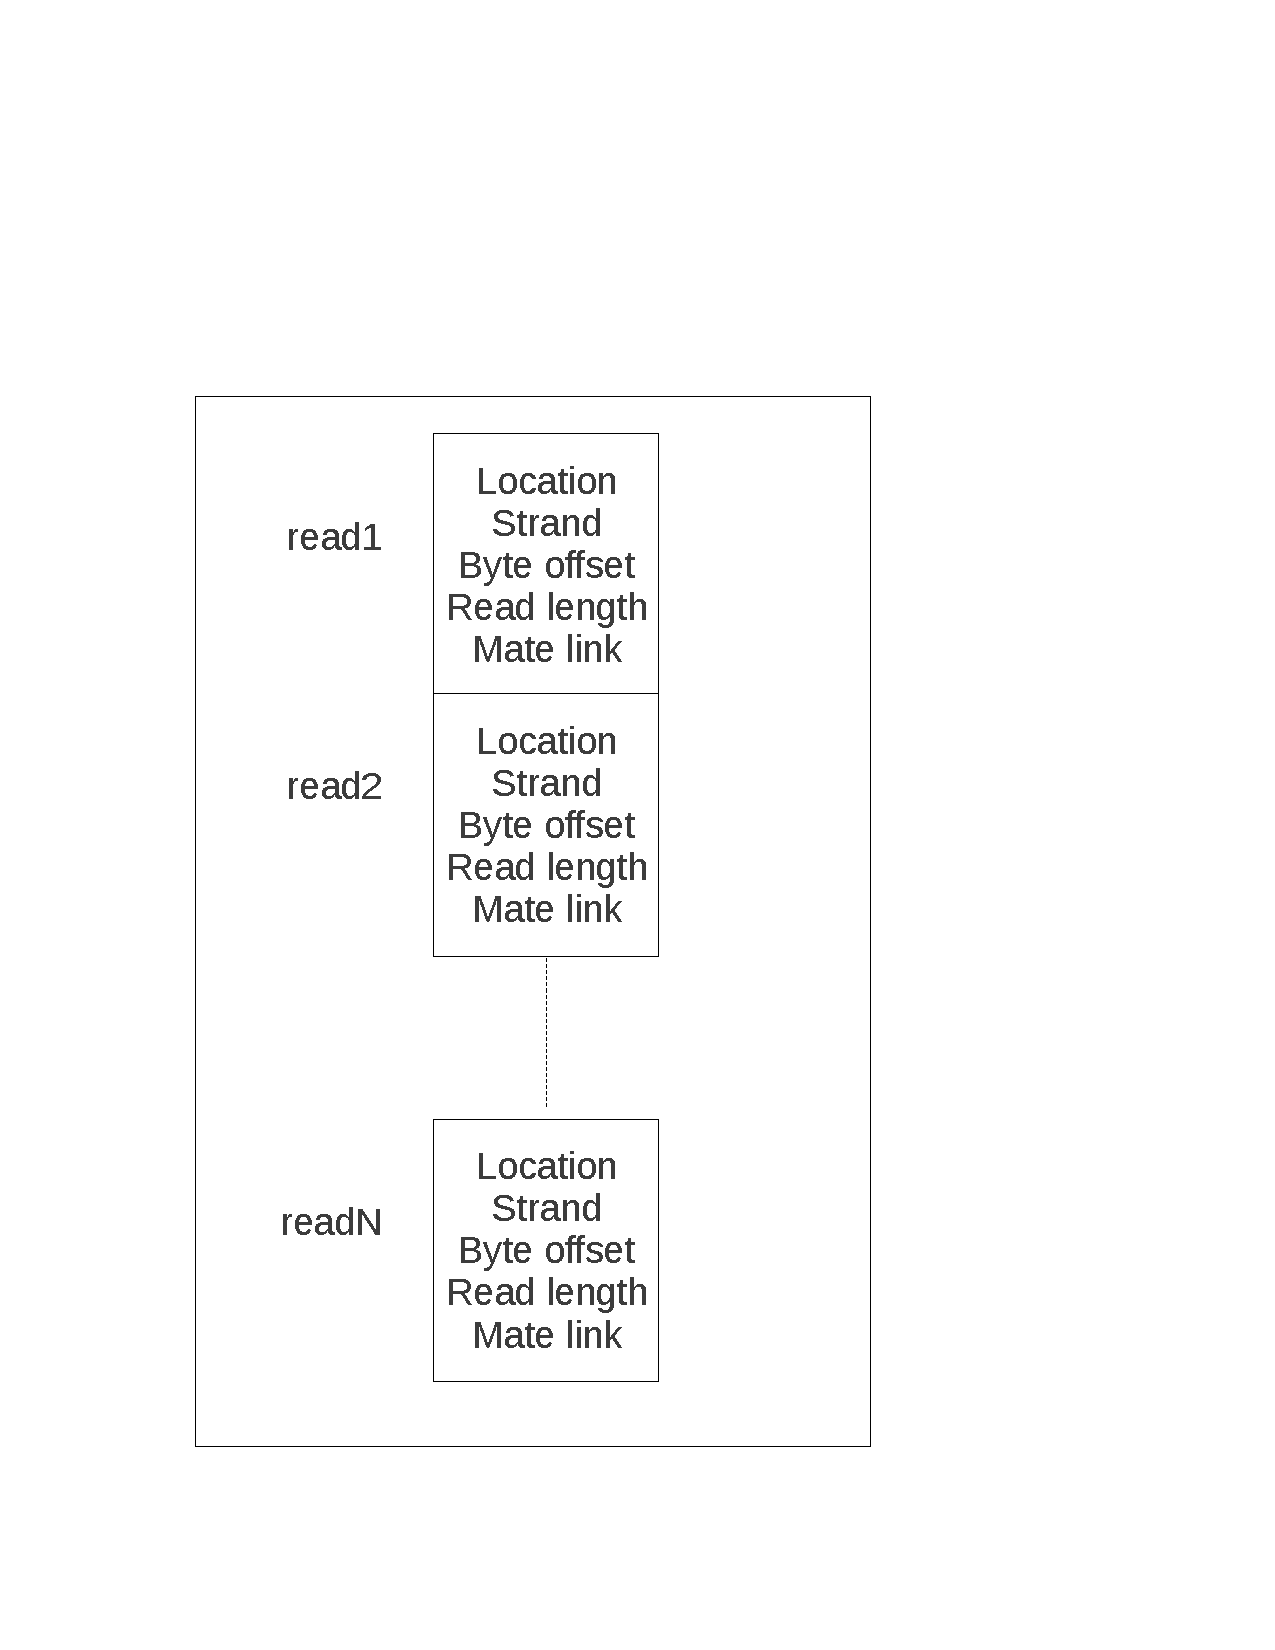
\includegraphics[trim = 30mm 30mm 60mm 40mm,
  clip,width=2in]{fig/indx_descr.pdf}
  \caption{{\footnotesize Our indexing scheme }}
  \label{fig:indx-descr}
\end{figure}


We claim that our index is small enough to fit in the main memory of
any computer. Since we use 8 bytes for the byte offset, 4 bytes for
the mapping location and the mate link, 10 bits for the read length
and 1 bit for the strand information, the size of the index of the set of
alignments of the largest chromosome (chr1) of coverage $35\times$ and
read length of $100$ is $1.5GB$. {\bf TODO in the current
implementation this is even worse. I use 2 bytes for the read length
and it seems that the indx is of size 2.3G. This is embarassing if we
compare it with the size of the bam file which is 6.1G. We might need
to compress further or go back to slimgene which gives similar
compression}.

The building of the index occurrs in a small time frame. In our
experiments, a dataset of approximately $90M$ reads from NA18507 
that map with chr1 requires $6$ minutes to create the index, while the
memory footprint of the execution does not exceed $2GB$ {\bf TODO:
verify that}.

\subsection{Searching for Ranges}
\label{sec:range}

Although the retrieval of reads that overlap with a given range is
easily implemented with the indexing scheme of Samtools, we choose to
use our existing index for such an implementation. In this way we simplify the
design by eliminating the necessity of maintaining multiple indexes.

The implementation of this query requires the knowledge of the byte
locations of the reads of the answer in the bam file. Thus we scan
sequentially the index up to the location of the entry of the first
read that overlaps with the given range. The desired byte offset is
the value of the {\em byte offset} field of the array.

Although this search on the index is more complex than the search that
samtools use, in practice the difference in time is negligible.
Obviously a sequential scan of N entries has a time complexity of O(N)
which is slowly from a lookup that samtools use which is of O(1).
However, the fetching of the actual reads from the disk eliminates the
overhead of the sequential search in the main memory.

\subsection{Retrieving Areas by Coverage}
\label{sec:coverage}
In this section we describe the implementation of the query: 
``{\em Given a constant $k$, find all regions of a chromosome which are
covered by at least $k$ reads}''. In addition we show why the
implementation with our index outperforms alternative implementations.

This query requires an auxiliary array of counters that keeps the
read counts in each position. The array has a length equal to the
length of the chromosome of interest and it is initialized to 0. Each
read increases the counters of those positions that overlap with it
and a backtracking step reports the areas of interest.

\fref{fig:coverage-example} shows the contents of the counters in an
imaginary scenario of a chromosome of length $10$ and reads of length
$2$. The value of each counter is the number of reads that overlap with 
its location. The backtracking for $k=0$ reports that areas $1$ and
$6-7$ are covered by $0$ reads. {\bf TODO: I haven't implemented the
coverage query in this way yet. This might change in the future}

\begin{figure}[hbt]
  \centering
  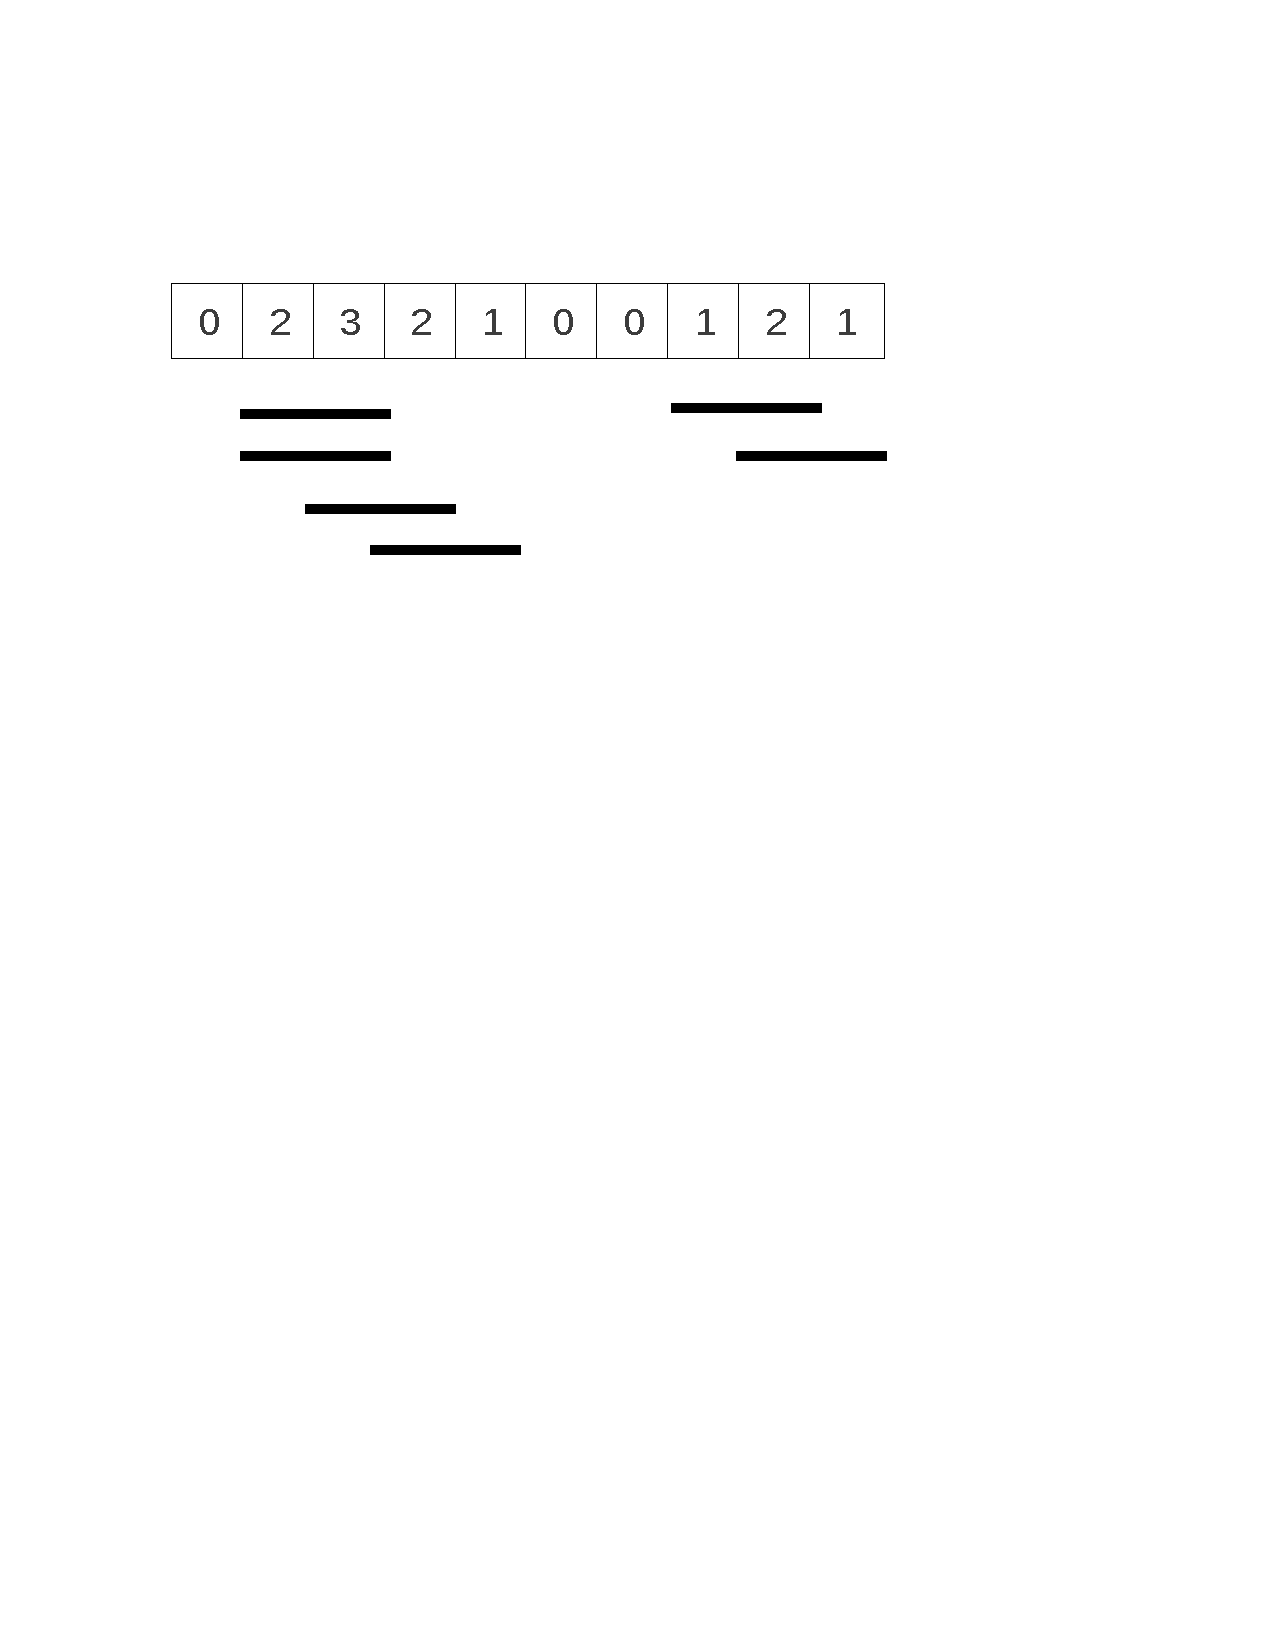
\includegraphics[trim = 15mm 185mm 60mm 40mm,
  clip,width=2in]{fig/coverage_example.pdf}
  \caption{{\footnotesize The auxiliary vector of counters of the
  coverage query.}}
  \label{fig:coverage-example}
\end{figure}

Of course this question can be easily answered with the pileup
function of samtools at the expense of efficiency. The pileup requires
more time to be built because it needs all the data of the input file.
Thus, the in memory manipulation of the index is more efficient. {\bf
TODO: will come back with real numbers}.

\subsection{Locating areas with discordant clones}
\label{sec:discordant}

In this section we explain how we implement the query: ``{\em Find all
regions that are covered by at least $k$ discordant clones}''. A user
can define any type of {\em discordancy} in the context of this query. 

The detection of the areas that are covered by multiple discordant
clones is proportional to the number of the discordant clones if we
model it after the balanced parenthesis problem. A left parenthesis is 
assigned for every leftmost coordinate of a discordant clone and a closing 
parenthesis is assigned for every rightmost coordinate of a discordant clone. 
Thus the area that is covered by at least $k$ discordant clones is the
area where $k$ or more parenthesis are open concurrently. Then the
solution requires a counter which increases each time a parenthesis is
open and decreases when a parenthesis closes. The regions of interest
are the areas for which the values of the counter are at least $k$.
Obviously, the number of the steps that are required by this algorithm
is equal to the number of reads that are involved in the discordant
clones.

As an example consider the discordant clones of
\fref{fig:disc-example-a}. \fref{fig:disc-example-b} shows the modeling
of the same clones with the use of parenthesis. Note that a
parenthesis opens at every position which is the starting point of a
clone and it closes at those positions that are the rightmost ends of
clones. The values of the counter appear in the bottom of this figure
and for $k=3$ the area of interest includes all positions whose value
is greater than $2$.

\begin{figure}[hbt]
  \centering
  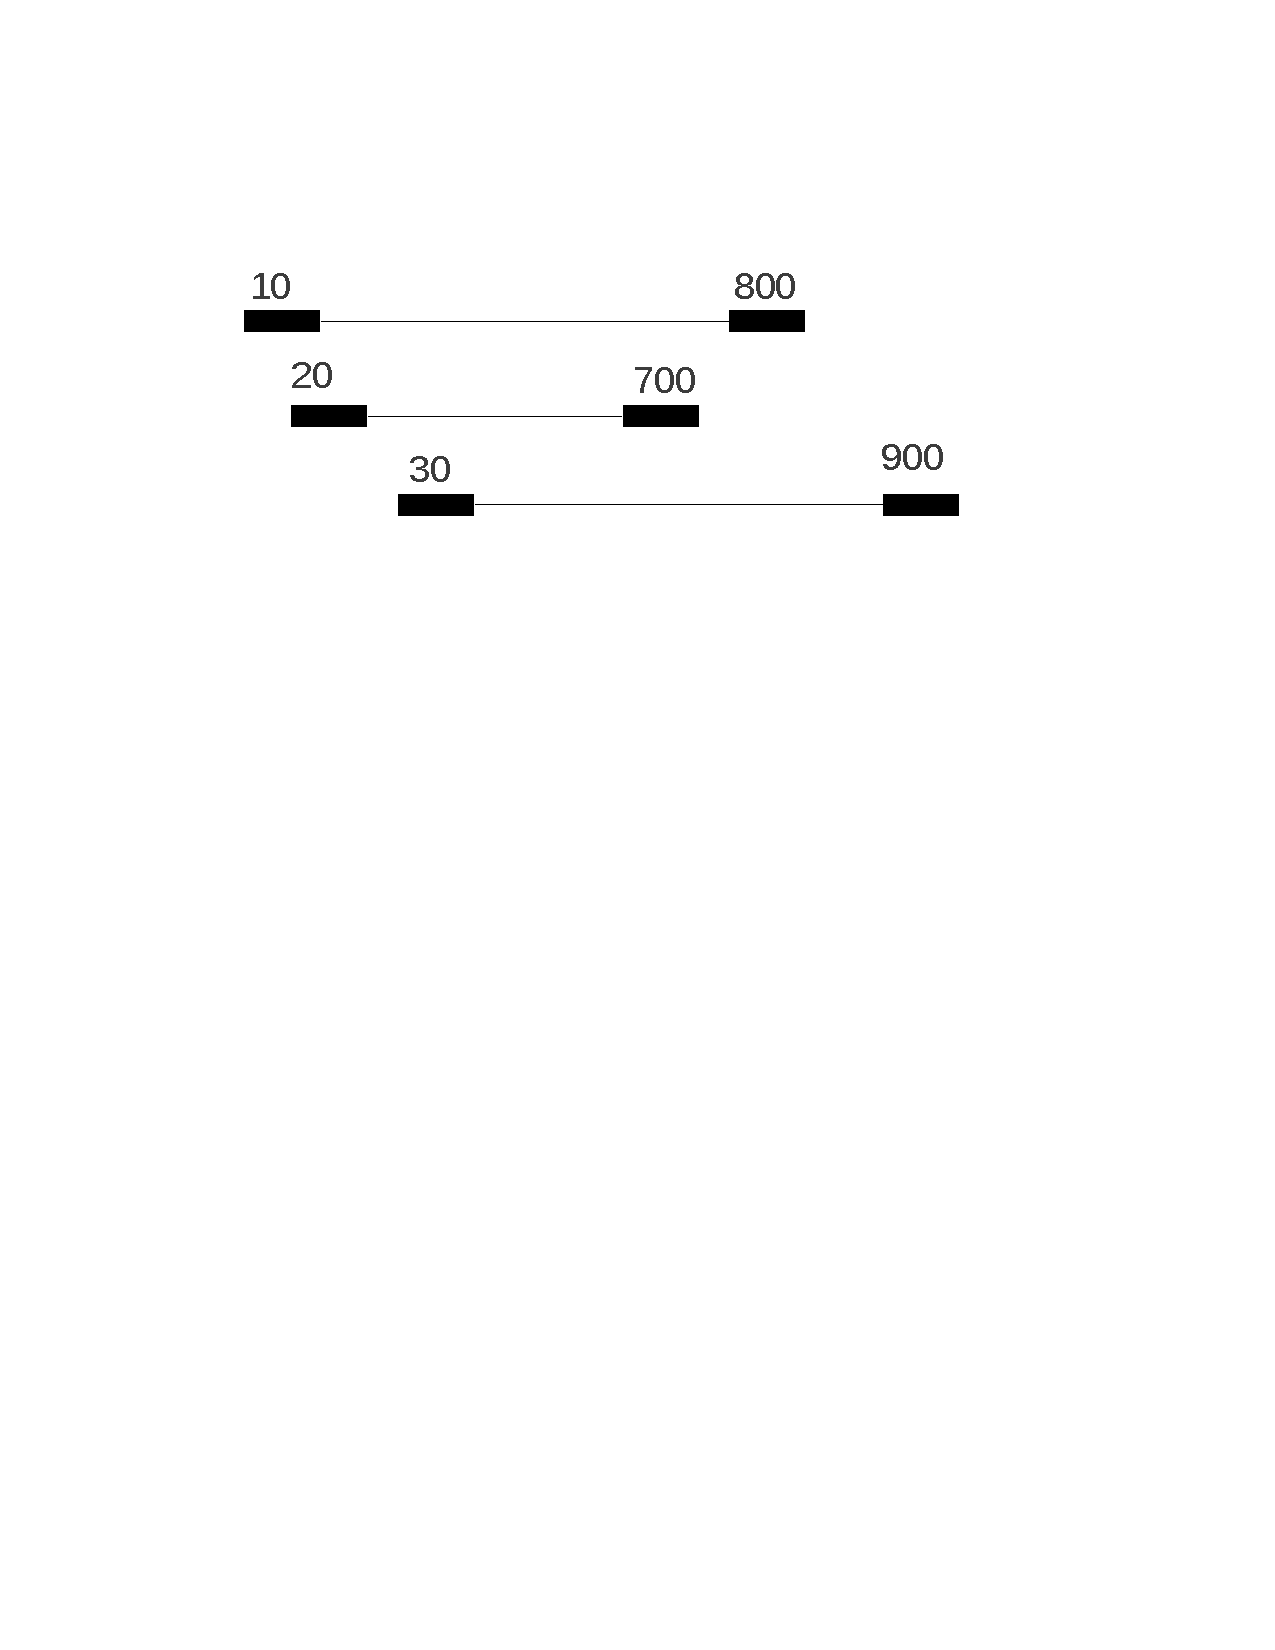
\includegraphics[trim = 30mm 190mm 55mm 40mm,
  clip,width=2in]{fig/disc_example_a.pdf}
  \caption{{\footnotesize A set of discordant clones.}}
  \label{fig:disc-example-a}
\end{figure}

\begin{figure}[hbt]
  \centering
  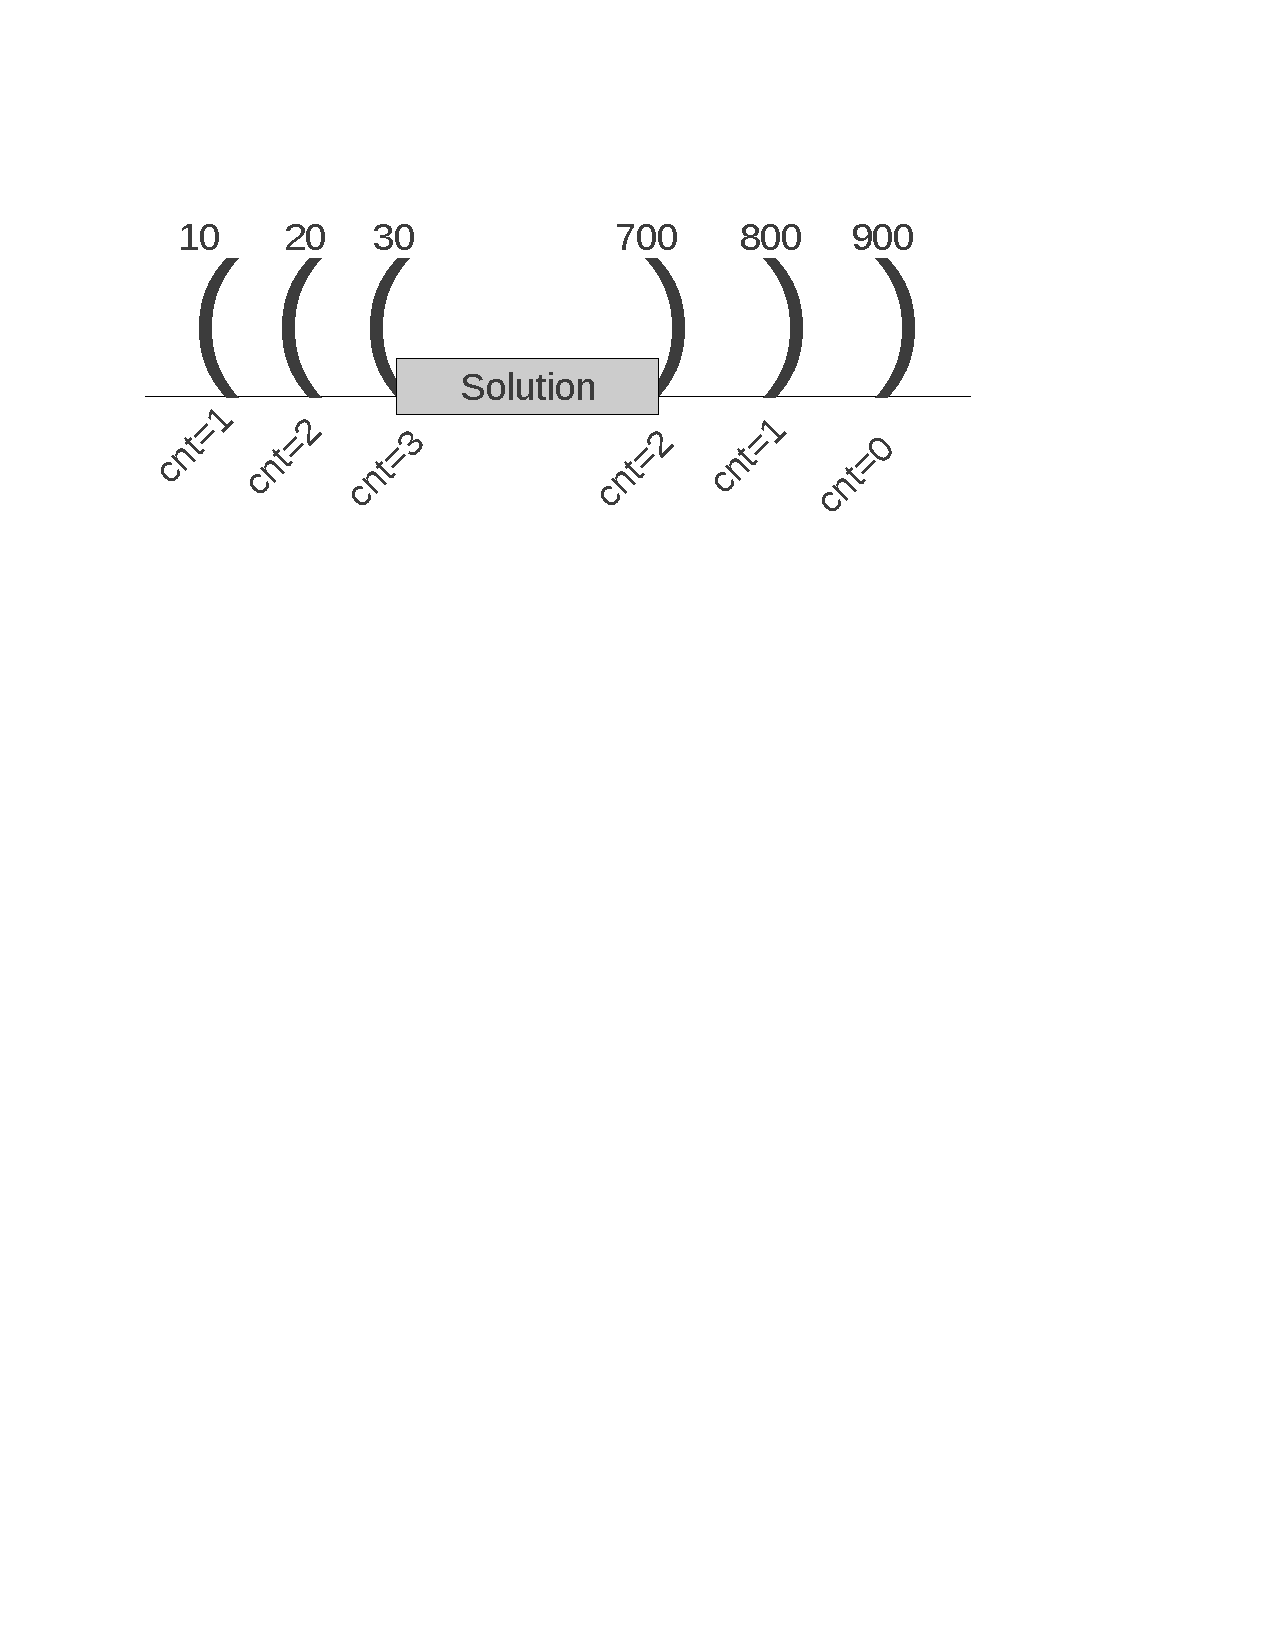
\includegraphics[trim = 25mm 190mm 55mm 30mm,
  clip,width=2in]{fig/disc_example_b.pdf}
  \caption{{\footnotesize The discordant clones are modeled
  parenthesis. The shaded area is the region which is covered by at
  least $3$ clones.}}
  \label{fig:coverage-example}
\end{figure}

\subsection{Creating a Haplotyping Graph}
\label{sec:haplograph}

In this section we describe how we implement the query:	``{\em Given a set 
of SNP loci find those pairs of reads that contain at least two of
them}''. More formally the query can be formalized as follows: {\bf
TODO: I will rewrite the following using hte algorithmic package}

\begin{itemize}
\item {\bf Input: } A set $I$ of positive integers.
\item {\bf Input: } A set $R$ of intervals of the form $\left(x_1,
x_2\right)\vee\left(x_3, x_4\right)$
\item {\bf Output: } A set $S \subset R$ such that $\forall r \in S
\exists m,n \in I and m,n \in r$.
\end{itemize}

{\bf TODO: Is there any bibliography that solves this problem with
interval trees? I would like to show that interval trees cannot do
better than our approach. If there is not such a thing available I can
give back of envelope calculations.}

An efficient implementation of this query involves a bit vector of of
the same length as the chromosome of which the elements of $I$ came
from. All positions of the bitvector that are also contained in $I$
get the value of $1$. An interval that represents a read is part of
the set $S$ if the bitvector contains $2$ or more ones in the
correspondent region.

Thus the problem is reduced to the problem of counting the number of
ones in a vector $v$. This is a well studied problem and the
number of ones of $v$ can be obtained by the number of iterations
according to which the value $v=v\&(v-1)$ is non zero. For example, if
we count the number of ones that appear in $v=5$ ($101$ in binary) in
the first iteration we have $v=5\&4=4$ and in the second iteration
$v=4\&3=0$. Thus the number of ones is $2$. 

The complexity of the algorithm is $O(|R|+|I|)$ since we count the
number of ones for all reads of $R$ and the total number of iterations
is going to be exactly equal to the number of ones of the bitvector.

\end{document}
